\section{Introduction}
\label{sec:intro}
\ihead{Introduction}
This project focuses on the development of a \ac{ML} model for short-term electricity demand forecasting. The analysis is restricted to the 50Hertz control area, which covers eastern Germany as well as the metropolitan region of Hamburg as depicted in Figure~\ref{fig:50hertz_region}. The main objectives are the construction of a dataset including relevant exogenous variables and the prediction of hourly electricity demand with a forecasting horizon of up to 24 hours. Accurate short-term load forecasts are essential for efficient grid operation, market planning, and maintaining overall system stability.

All source code and datasets are publicly available in
our GitHub repository under the MIT license\footnote{\href{https://github.com/lar-tech/electricity-demand-forecasting}{github.com/lar-tech/electricity-demand-forecasting}}.
\begin{figure}[H]
    \centering
    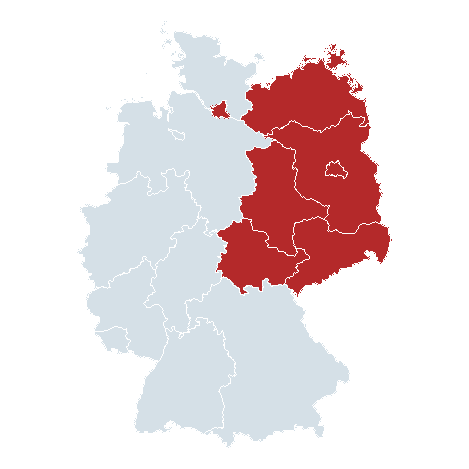
\includegraphics[width=0.35\linewidth]{figures/50hertz_region.pdf}
    \caption{50Hertz control area marked in red.}
    \label{fig:50hertz_region}
\end{figure}